%!TEX root = ../../report.tex
\chapter{Cost Interpretation}
\ref{chapter:cost_interpretation}
This chapter describes how the learned dynamic behaviors of the environment can be converted to a map of good features and areas to avoid when navigating. Specifically the following aim is considered:

\begin{enumerate}
    \setcounter{enumi}{2}
    \item Improved localization with a continuously adapted map of good features
\end{enumerate}

The dynamic learner represents the dynamic map of the environment by the parameters in PMAC. These parameters are not directly usable by the localization and navigation systems. In order to provide a usable map to these subscribers an interpretation of the parameters is necessary. This is handled by the Cost interpretor which is shown in relation to the rest of the Dymamic mapping system in figure \ref{fig:cost_overview}.

\begin{figure}[htbp]
	\centering
	\includegraphics[scale=1]{chapters/cost_interpretation/figures/cost_overview.eps}
	\caption{Cost interpretation in the dynamic mapping system}
	\label{fig:cost_overview}
\end{figure}

%!TEX root = ../../report.tex
\section{The Dynamic Mapping on MiR-100}
In the test platform used in this project the output required by the subscribing systems is a costmap. This grid represents the world as cells, each with a value for the cost of traversing it. 
The system is built to be run with the MiR-100 robot. This involves constructing and interfacing the Dynamic mapping system with the ROS setup on the robot. The developed system is shown in figure \ref{fig:mir_interface} along with the ROS nodes it interacts with. 

\begin{figure}[htbp]
	\centering
	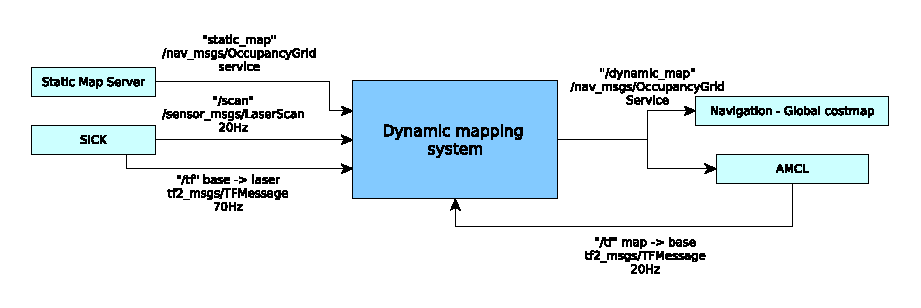
\includegraphics[width=1\linewidth]{chapters/cost_interpretation/figures/dynamic_map_mir_interface.eps}
	\caption{The Dynamic mapping system with connected nodes and interface.}
	\label{fig:mir_interface}
\end{figure}

The Dynamic mapping system receives a static map from the Static Map Server in order to initialize the Dynamic learner. This is only done at startup. The primary input for the Dynamic mapping system is the laser scan data provided by the SICK node and the pose of the robot in the world provided by AMCL. The pose of the scanners on the robot is provided by the SICK system. 
The Dynamic mapping system is based on the ROS implementation of the Layered costmap \cite{lu2014layered}. Each layer maintains its own costmap and these are combined to produce the output costmap. Figure \ref{fig:dynamic_map_server_internal} shows the elements of the Dynamic mapping system and the flow of data. The layered costmap in the Dynamic mapping system contains three layers; Activity, User priority and Blueprint layer. 

\begin{figure}[htbp]
	\centering
	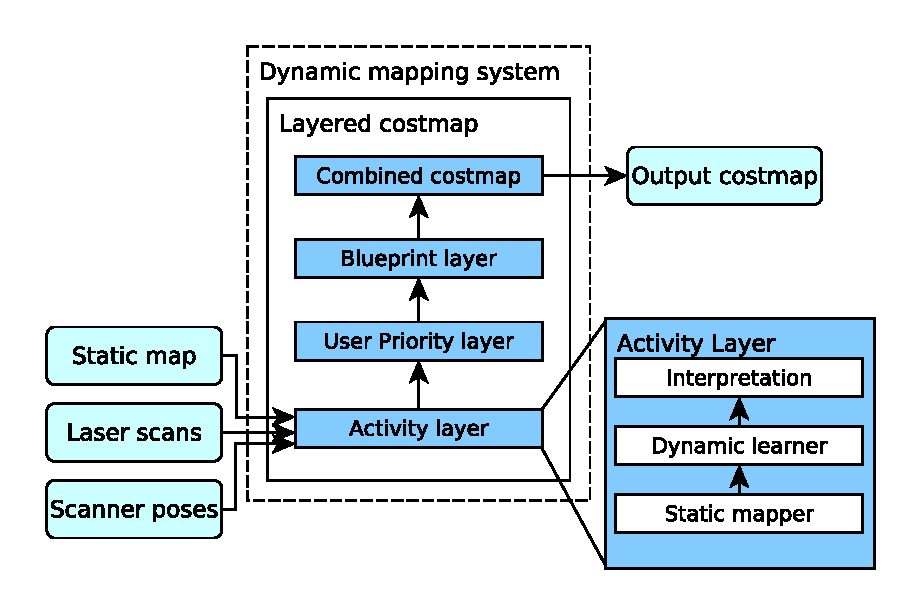
\includegraphics[scale=0.7]{chapters/cost_interpretation/figures/implementation_overview.eps}
	\caption{The Dynamic Map Server internal components}
	\label{fig:dynamic_map_server_internal}
\end{figure}


The Activity Layer is the primary layer and handles the mapping, learning of the dynamics and interpretation of the dynamics. It delivers a costmap that should contain the learned static obstacles with a high cost and dynamic obstacles with a cost appropriate to its dynamic. 

The second layer in the Dynamic Map Server is the User priority layer. This layer is designed override the cost of certain cells. This could be used to ensure that selected areas are avoided or preferred based on the user requirements. 

The Blueprint layer can contain walls and structural elements of the environment.
These elements are expected to be absolutely stationary for the entire time of operation.
This can be used to avoid any possible erosion, of the walls in the map representation, due to erroneous localization.
Another benefit of the Blueprint layer is to limit the risk of unintended feedback by wrong mapping due to  erroneous localization.
The Blueprint layer is implemented as an instantiation of the Static Map Layer \cite{lu2014layered}. 

Because the Dynamic mapping system is implemented as a layered costmap it is possible add new layers by means of a simple ROS API \cite{plugin_lib}. This could be layers for other sensors, like SONAR \cite{range_sensor_layer} or 3D cameras.
%!TEX root = ../../report.tex
\section{Feature map for Monte Carlo localization}
For the Monte Carlo localization the features that is desired are static object like buildings, heavy machinery, etc. These share the property of not moving. The elements added for the localization should therefore be cells that have been very static. In the interpretation step each cell is classified as static or non-static. Cells that have been classified as static are given the maximum value, lethal, in the costmap. 
The parameters available for classification are:
\begin{itemize} 
\item Sum of occupied scores
\item Sum of free scores
\item Sum of exit events
\item Sum of entry events
\item Previous observation
\item \(\lambda_{exit}\) - estimated by exit events and occupied scores
\item \(\lambda_{entry}\) - estimated by entry events and free scores
\end{itemize}

We propose a simple classifier that bases its decisions on \(\lambda_{exit}\), the sum of occupied scores and the sum of free scores.  \(\lambda_{exit}\) is chosen because one of the primary requirements is that the probability of the cell to switch to free should be very low for static obstacles. The two sums are used to ensure that the cells has been more occupied than free. 
The classification rules was determined based on simulation as well as real world data. In figure \ref{fig:amcl_classifier} is shown the classification results as well as the ground truth. Figure \ref{fig:amcl_classifier:worst} shows a bad classifier that includes all the dynamic obstacles. The results from the chosen classifier are shown in figure \ref{fig:amcl_classifier:chosen}. In the result almost all of the dynamic obstacles are removed. It was not possible to adjust the limits to suppress the remaining dynamical obstacles without damaging the true walls. In the simulation the robot drove from the top-right corner to the bottom-left. This means that the amount of data from the two remaining corners are very limited. 

%% FIGURE - CLASSIFICATIONS
\begin{figure}[htbp]
	\label{fig:amcl_classifier}
	\begin{subfigure}{.5\textwidth}
		\centering
		\includegraphics[width=1\linewidth]{chapters/cost_interpretation/figures/occ_above_0_classifier.png}
		\caption{Obstacles: \(\Sigma state_{occ} > \Sigma state_{free}\)}
		\label{fig:amcl_classifier:worst}
	\end{subfigure}
	\qquad
	\begin{subfigure}{.5\textwidth}
		\centering
		\includegraphics[width=1\linewidth]{chapters/cost_interpretation/figures/chosen_classifier.png}
		\caption{Obstacles: \(\Sigma state_{occ} > 2 \cdot \Sigma state_{free}\) and \(\lambda_{exit} < 0.15\) }
		\label{fig:amcl_classifier:chosen}
	\end{subfigure}\\[1ex]
	\begin{subfigure}{1\textwidth}
		\centering
		\includegraphics[width=.5\linewidth]{chapters/cost_interpretation/figures/dynamic_area_web.png}
		\caption{Ground truth map}
		\label{fig:amcl_classifier:groundtruth}
	\end{subfigure}
	\caption{Results of different classifier rules and the true map}
    \label{fig:amcl_classifier}
\end{figure}

%!TEX root = ../../report.tex
\section{Costmap for Path Planning}
\label{sec:cost_interpretation_path_planning}
The path planning uses the costmap to determine the path with the lowest cost while avoiding lethal obstacles. 
The path planner uses lethal as well as non-lethal costs to accomplish this. 
Therefore, the dynamic obstacle should be represented to help guide the path planning away from obstacles that might obstruct the path and possibly cause a re-planning. 
Because path planning is most likely handled without observing most of the path the cost of cells have to be predicted. 
The Markov model used in the Dynamic learner is well suited to estimate the probabilities for being in the free or occupied state. 
Given the time since the last observation it is possible to calculate the number of steps the Markov chain must go through to project the state to the current time.
The predictions are performed from the estimated occupancy probability, which is updated with new measurements.

\subsection{Occupancy Estimation Update}
A simple update of the estimated occupancy probability would be to override it with the latest observation.  
A problem with this is uncertainty in observations. 
If an observation is very uncertain ($\approx0.5$), it carries very little information and therefore not very suitable to be used in the forward projection. 
As it is not desirable to use such uncertain values as basis for the forward projection, an update and predict scheme is used.
Each time a new value is received the current occupancy probability estimate, \(\hat{p}_{occ}(t)\), is updated as shown in equation \ref{eq:cost_update}.
%
\begin{equation}
\label{eq:cost_update}
\hat{p}_{occ}(t) = \hat{p}_{occ}(t-1) +  2  \left\| p_{occ} - 0.5 \right\| \cdot \left[p_{occ} - \hat{p}_{occ}(t-1) \right]  
\end{equation}
%
The correction value is the difference between the new measurement and the previous estimate.
This is weighted according to the certainty in the new observation.  
Figure \ref{fig:cost_update} shows an example of the update method for the \(\hat{p}_{occ}\). 
\begin{figure}[htbp]
	\centering
	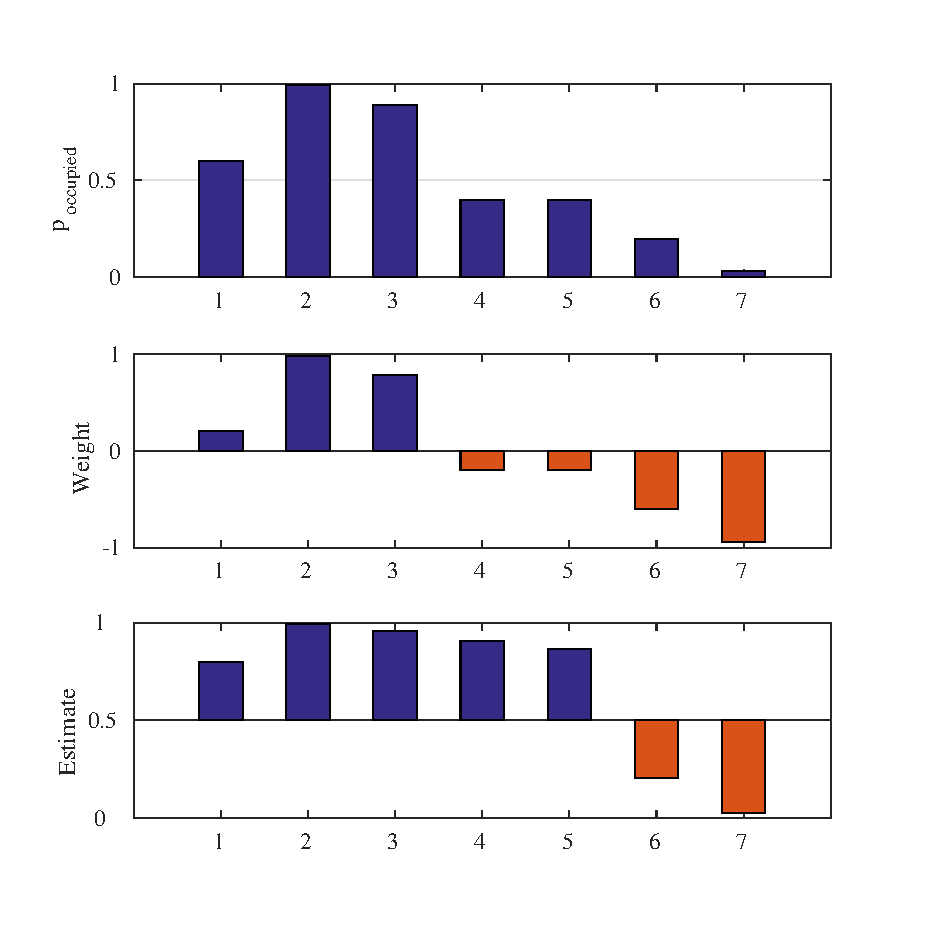
\includegraphics[width=1\linewidth]{chapters/cost_interpretation/figures/update}
	\caption{Update of the estimated occupancy. Sign in weight indicates free or occupied, positive is occupied. }
	\label{fig:cost_update}
\end{figure}
\todo{axis x -> t}
It is seen in figure \ref{fig:cost_update} that the uncertain free values does not cause a great shift in the estimated occupancy value. When the free observations become increasingly certain a significant change is observed. 

\subsection{Occupancy Prediction}
The predict steps are performed when a new map is to be generated. At this time all cells are projected forward from their last observed time to the current time. This is done by using the estimated occupancy as the initial distribution and then projecting forward a number of steps according to the time difference between last observation and the current time.
Equation \ref{eq:markov_project} shows the $n$ step projection of the estimated occupancy probability.
\begin{equation}
\label{eq:markov_project}
\begin{bmatrix}
1-p_{proj} & p_{proj}
\end{bmatrix}
=
\begin{bmatrix}
1-\hat{p}_{occ} & \hat{p}_{occ}
\end{bmatrix}
\cdot
\begin{bmatrix}
1 - \hat{\lambda}_{entry} & \hat{\lambda}_{entry}\\ 
\hat{\lambda}_{exit} & 1- \hat{\lambda}_{exit}
\end{bmatrix}^n
\end{equation}
If the number of steps to project is larger than five, then the estimate is not used. Instead the stationary distribution in  equation \ref{eq:long_term} determines the final occupancy probability \cite{Meyer-Delius2012}.
\begin{equation}
	\label{eq:long_term}
	p_{stationary} = \frac{1}{\lambda_{entry} + \lambda_{exit}} \cdot \lambda_{entry}
\end{equation}

Figure \ref{fig:cost_predict} shows the projection of a cell with the Markov parameters \(p_{exit} = 0.13 \) and \(p_{entry} = 0.52 \). 
The initial probability estimate is the last estimate from figure \ref{fig:cost_update}. 
It is clear that in this case, it does not take many forward projection until it converges close to the long term. 

\begin{figure}[htbp]
	\centering
	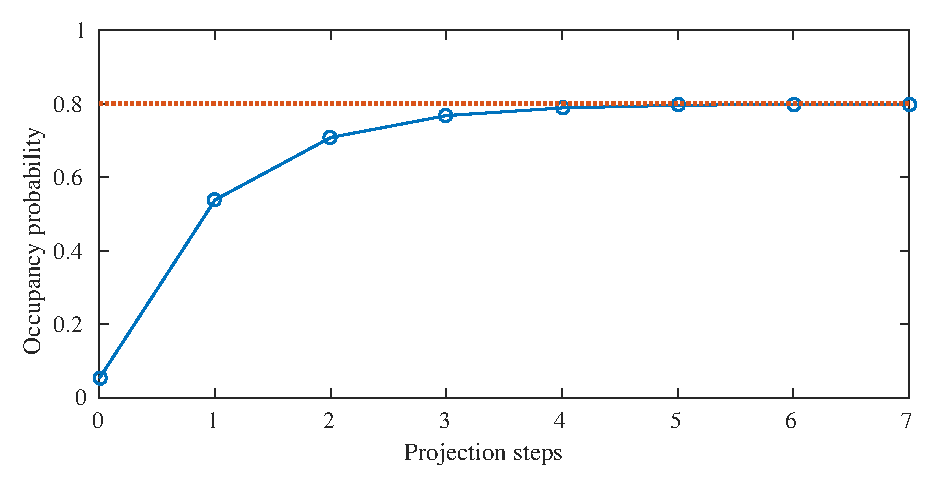
\includegraphics[width=1\linewidth]{chapters/cost_interpretation/figures/projection}
	\caption{Prediction of occupancy. Markov parameters: \(\lambda_{entry} = 0.52\), \(\lambda_{exit} = 0.13\)}
	\label{fig:cost_predict}
\end{figure}

\subsection{Converting Probability to Cost}
The cost assigned to the costmap is controlled by the function $\phi(p)$. Its input is the occupancy probabilities calculated by the prediction methods.
The function scales the probability into the cost range assigned to dynamic obstacles.
The cost $\kappa$ depends on $n$ as shown in equation \ref{eq:cost_conversion}.
The nature of the function $\phi$ depends on the path planner and demands for the path. 

\begin{equation}
\label{eq:cost_conversion}
\kappa = 
\begin{cases}
\phi(p_{proj}), & \text{if } n \le 5
\\
\phi(p_{stationary}), & \text{otherwise}
\end{cases}
\end{equation}
\section{Summary}
This chapter investigated the interpretation of the learned dynamics into a representation usable by localization and navigation systems.
The Dynamic mapping system was integrated on the MiR-100 as a layered costmap which enable integration of user priorities and blueprint maps as well as the learned dynamics.
The translation from the dynamic representation to costs was split in two.
The map for localization only contains obstacle classified as static.
The costmap used for path planning is determined from the probability for occupancy and the dynamics.
This is done by maintaining an updated estimate of the occupancy and predicting the occupancy to come. 
The estimated occupancy probability is updated with new measurements while considering the confidence in it.
For prediction the Markov representation is used to project the estimated occupancy from the time of the last observation to the time of planning.

The classification and projection is incorporated into the Dynamic mapping system in the Cost interpretor section as shown in figure \ref{fig:cost_interpretor_detail}.

\begin{figure}[htbp]
	\centering
	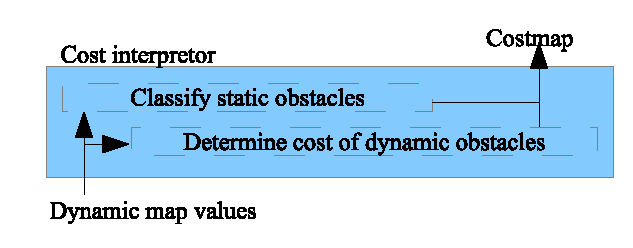
\includegraphics[scale=1]{chapters/cost_interpretation/figures/cost_detail}
	\caption{The Cost interpretor section of the Dynamic mapping system.}
	\label{fig:cost_interpretor_detail}
\end{figure}





